\documentclass[10pt]{article}

% Lines beginning with the percent sign are comments
% This file has been commented to help you understand more about LaTeX

% DO NOT EDIT THE LINES BETWEEN THE TWO LONG HORIZONTAL LINES

%---------------------------------------------------------------------------------------------------------

% Packages add extra functionality.
\usepackage{
	times,
	graphicx,
	epstopdf,
	fancyhdr,
	amsfonts,
	amsthm,
	amsmath,
	algorithm,
	algorithmic,
	xspace,
	hyperref}
\usepackage[left=1in,top=1in,right=1in,bottom=1in]{geometry}
\usepackage{sect sty}	%For centering section headings
\usepackage{enumerate}	%Allows more labeling options for enumerate environments 
\usepackage{epsfig}
\usepackage[space]{grffile}
\usepackage{booktabs}
\usepackage{amsmath}
\usepackage[super]{nth}
\usepackage{array}

% This will set LaTeX to look for figures in the same directory as the .tex file
\graphicspath{.} % The dot means current directory.

\pagestyle{fancy}

\lhead{\YOURID}
\chead{\MyLang: Language Specification}
\rhead{\today}
\lfoot{CSCI 334: Principles of Programming Languages}
\cfoot{\thepage}
\rfoot{Spring 2020}

% Some commands for changing header and footer format
\renewcommand{\headrulewidth}{0.4pt}
\renewcommand{\headwidth}{\textwidth}
\renewcommand{\footrulewidth}{0.4pt}

% These let you use common environments
\newtheorem{claim}{Claim}
\newtheorem{definition}{Definition}
\newtheorem{theorem}{Theorem}
\newtheorem{lemma}{Lemma}
\newtheorem{observation}{Observation}
\newtheorem{question}{Question}

\setlength{\parindent}{0cm}
%---------------------------------------------------------------------------------------------------------

% DON'T CHANGE ANYTHING ABOVE HERE

% Edit below as instructed
\newcommand{\YOURID}{Angela + Catherine}	% Replace "Your Name Here" with your name
\newcommand{\MyLang}{DigiWeave}	% Replace MyLang with your language name #

\begin{document}

\vspace{\baselineskip}	% Add some vertical space

% Refer to the lab handouts to determine what should go in each of these sections.  Each lab is additive.  So lab 8 should include everything you wrote in lab 7.  Lab 9 should include everything you wrote in lab 8, etc.

\section{Introduction}

    Our language is essentially a friendship bracelet pattern generator. It will allow users to design their own patterns and test out whether they would actually be feasible to create beforehand (ex. no gaps in knots, strings end up in right position, etc.). Making friendship bracelets is also something a lot of people do, so we feel like a pattern generator would be a useful tool to have. 
		
	\vspace{\baselineskip}
	
	We think this would make a worthwhile programming language because if designed correctly, it will allow the generation of (possibly) infinite designs, fostering creative expression through the aid of technology. Also, we hope to make the language relatively simple and user-friendly (and perhaps with some sort of graphical interface) so that anyone, regardless of coding experience, can design with it :).

\section{Design Principles}

    This language would definitely be guided by simplicity and clarity to keep the non-technical user in mind. We would also want the language to translate naturally from the physical art of bracelet making (ex. for a double right knot, maybe the user would type DR or something). The language would be flexible enough to allow the user's creativity to shine, while remaining relatively straight forward and easy to understand.
		
	\vspace{\baselineskip}
	
	If possible, it would be cool to create an interface that simulates a digital bracelet with the user's finished pattern at the end too, so they can really visualize what it would look like. We definitely also want to provide support for users in the cases of invalid expressions, syntax errors, or other things like that. 

\section{Example Programs}

    To run these example programs, type \verb|dotnet run ../../examples/example-1.fbp| on the command line from inside the lang directory. Replace "1" with "2" or "3" to try the other examples. The code and output is shown below. We are still working on the svgs but the evaluator output should match.
    
    \vspace{\baselineskip}

	Example 1: Two row pattern
	\begin{center}
    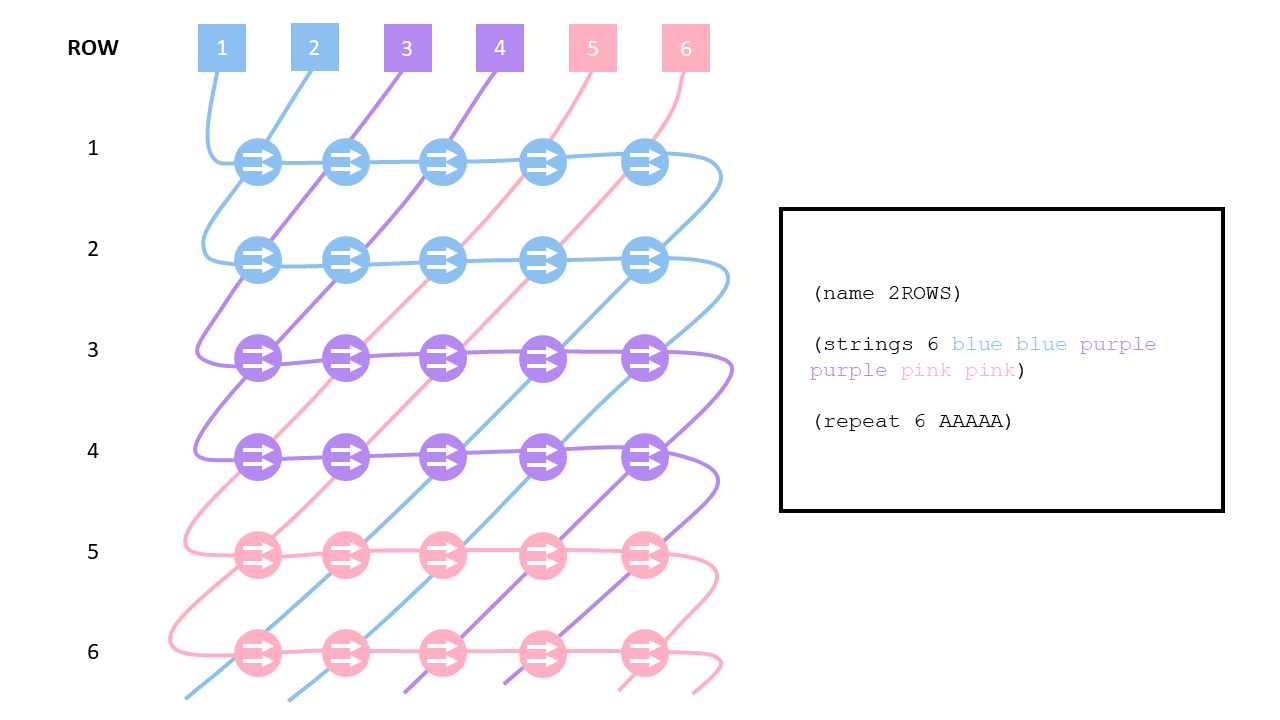
\includegraphics[width=\linewidth]{images/example1.png}
    \end{center}
    
    Evaluator output:
    \begin{verbatim}
Pattern Name: 2ROWS

Row
1   CornflowerBlue >> CornflowerBlue >> CornflowerBlue >> CornflowerBlue >> 
    CornflowerBlue >>
2   CornflowerBlue >> CornflowerBlue >> CornflowerBlue >> CornflowerBlue >> 
    CornflowerBlue >>
3   Coral >> Coral >> Coral >> Coral >> Coral >>
4   Coral >> Coral >> Coral >> Coral >> Coral >>
5   BurlyWood >> BurlyWood >> BurlyWood >> BurlyWood >> BurlyWood >>
6   BurlyWood >> BurlyWood >> BurlyWood >> BurlyWood >> BurlyWood >>
    \end{verbatim}
    
    Example 2: Arrow pattern
	\begin{center}
    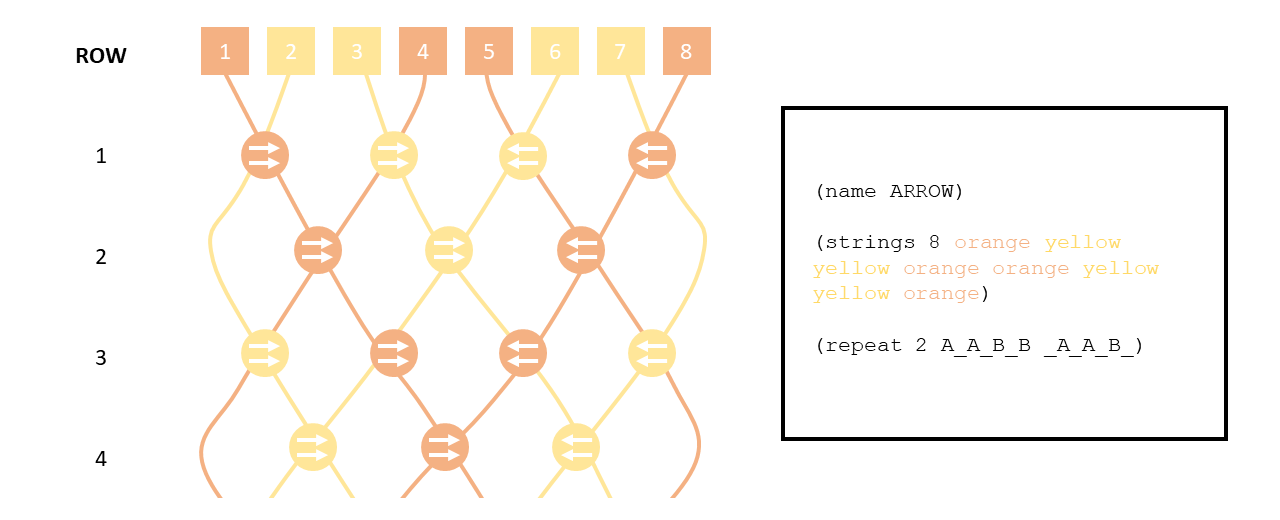
\includegraphics[width=\linewidth]{images/example2.png}
    \end{center}
    
    Evaluator output:
    \begin{verbatim}
Pattern Name: ARROW

Row
1   LightPink >>  _ LightSeaGreen >>  _ LightSeaGreen <<  _ LightPink <<
2    _ LightPink >>  _ LightSeaGreen >>  _ LightPink <<  _
3   LightSeaGreen >>  _ LightPink >>  _ LightPink <<  _ LightSeaGreen <<
4    _ LightSeaGreen >>  _ LightPink >>  _ LightSeaGreen <<  _
    \end{verbatim}
    
    Example 3: Heart pattern
	\begin{center}
    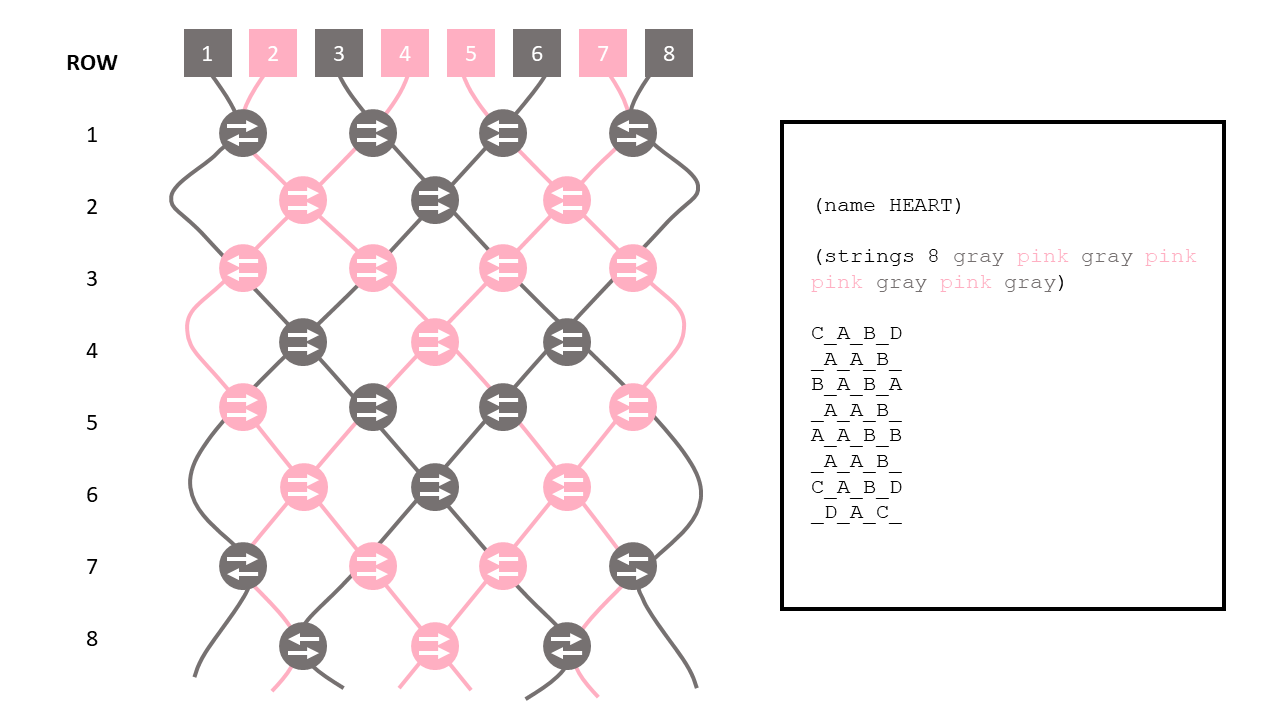
\includegraphics[width=\linewidth]{images/example3.png}
    \end{center}
    
    Evaluator output:
    \begin{verbatim}
Pattern Name: HEART

Row
1   PeachPuff >  _ PeachPuff >>  _ PeachPuff <<  _ PeachPuff <
2    _ PaleVioletRed >>  _ PeachPuff >>  _ PaleVioletRed <<  _
3   PaleVioletRed <<  _ PaleVioletRed >>  _ PaleVioletRed <<  _ PaleVioletRed >>
4    _ PeachPuff >>  _ PaleVioletRed >>  _ PeachPuff <<  _
5   PaleVioletRed >>  _ PeachPuff >>  _ PeachPuff <<  _ PaleVioletRed <<
6    _ PaleVioletRed >>  _ PeachPuff >>  _ PaleVioletRed <<  _
7   PeachPuff >  _ PaleVioletRed >>  _ PaleVioletRed <<  _ PeachPuff <
8    _ PeachPuff <  _ PaleVioletRed >>  _ PeachPuff >  _
    \end{verbatim}

\section{Language Concepts}

    	To write programs in this language, a user should understand the basic properties of a friendship bracelet. Essentially, a bracelet is made up of a repeated pattern, which is made up of rows, each of which consists of a certain combination of knots. There are 4 main knots: the double right knot, double left knot, right-left knot, and left-right knot. Rows can be repeated to form the pattern, or they can all be unique combinations of knots.
		
		\vspace{\baselineskip}
		
		Each bracelet also has a specified number of strings, each of which can be any color. The strings have an original order to start the pattern, but usually will move around as rows are constructed (based on which knots are used and in what order). See example programs above for a basic visualization of these concepts.

\section{Syntax}

    The syntax of this language is essentially as follows:
	\begin{itemize}
	    \item The overall program creates a \textbf{pattern}. A pattern is made up of:
	    \begin{itemize}
	        \item \textbf{Properties} which consist of
	        \begin{itemize}
	            \item The pattern's \textbf{name}
	            \item 1+ \textbf{strings}, each having a specified color and start position.
	        \end{itemize}
	        \item 1+ \textbf{Blocks} of 1+ rows. Blocks may or may not be repeated. In examples 1 and 2, there is 1 repeated block. In example 3, there is 1 block but it is not repeated. 
	        \begin{itemize}
	            \item Each \textbf{row} consists of 1+ \textbf{knots}, which are specified by one of the 4 valid knots (see the \textit{Language Concepts} section above for more details). To simplify things, the user will use the characters "A" "B" "C" and "D" to denote the knots, and "\_" to skip a string (aka. basically an "empty knot").
	        \end{itemize}
	    \end{itemize}
	    
	    \item In short, a pattern must contain a \textbf{name}, \textbf{strings} (with assigned colors), and at least 1 \textbf{row} of knots.
	\end{itemize}
	
    \vspace{0.5em}
	A diagram summarizing the syntax is given below.
	
	\begin{center}
    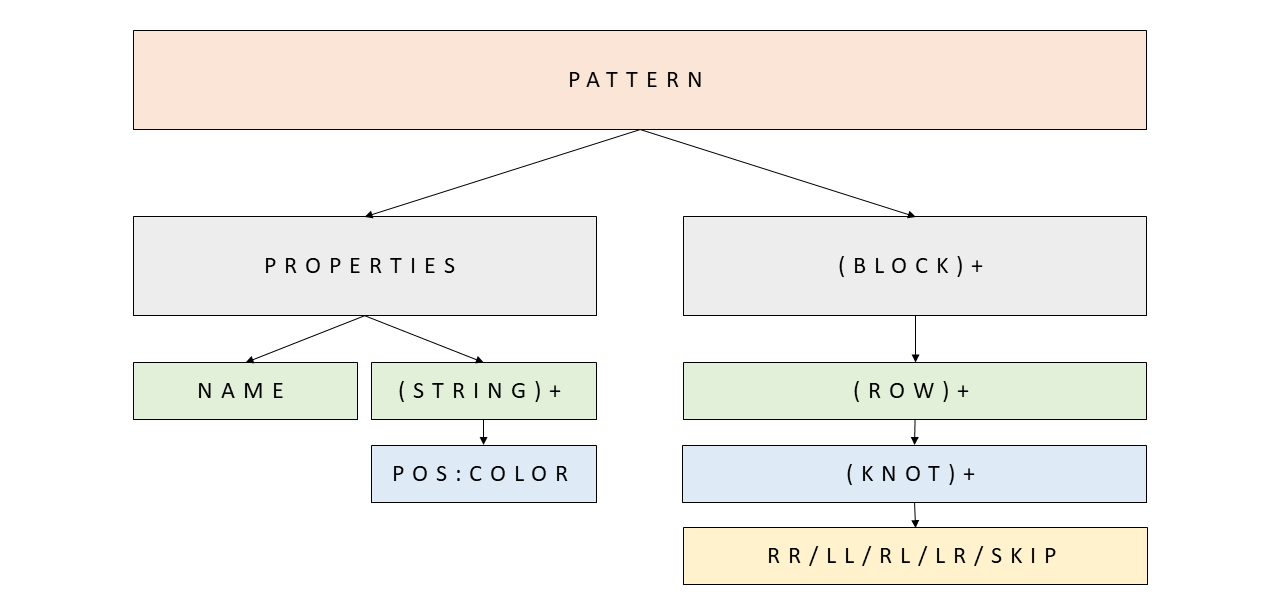
\includegraphics[width=\linewidth]{images/syntax.png}
    \end{center}
	
	Here is the equivalent, formal definition of the grammar in Backus-Naur form:
	
	\begin{verbatim}
<pattern> ::= <name> <strings> <comp>+
   <name> ::= string
<strings> ::= num <string>+
   <comp> ::= <block>
           | (repeat num <comp>+)
 <string> ::= any valid alphanumeric string
  <block> ::= <row>+
    <row> ::= <knot>+
   <knot> ::= RR | LL | RL | LR | SKIP
    <num> ::= n in Z+ (aka. any positive integer)  
	\end{verbatim}


\section{Semantics}
    
    See the next page for a table that summarizes the semantics of our program.
    
    \begin{table}
        \begin{tabular}{c|c|c|c|c} 
        \textbf{Syntax} & \textbf{Abstract Syntax} & \textbf{Type} & \textbf{Prec./Assoc.} & \textbf{Meaning} \\
        \hline
        n & n of int & int & n/a & \multicolumn{1}{m{4cm}}{N is any positive integer. A primitive used in the repeat and setup operations (see below for more details).} \\
        \hline
        "A", "B", "C", "D", "\_" & \multicolumn{1}{m{2.5cm}|}{Knot = RR $|$ LL $|$ RL $|$ LR $|$ SKIP of char} & char & n/a & \multicolumn{1}{m{4cm}}{Knots are primitives. We use these five chars to represent the four valid knots and the skip knot in the pattern.} \\
        \hline
        "ABCD\_" & Row of Knot list & Knot list & n/a & \multicolumn{1}{m{4cm}}{Rows are lists of knots. Since knots are basically chars, rows are sequences of chars, or strings.} \\
        \hline
        "AAA BBB" & Block of Row list & Row list & n/a & \multicolumn{1}{m{4cm}}{Blocks are lists of rows. Blocks are a type of Comp, short for component.} \\
        \hline
        (repeat n X X ... X) & \multicolumn{1}{m{2.5cm}|}{RepeatOp of int * Comp list} & int * Comp list & 1/left & \multicolumn{1}{m{4cm}}{The repeat operation will process the specified Comp n times. RepeatOp itself is also a type of Comp.} \\
        \hline
        (name "Name") & NameOp of string & string & 1/left & \multicolumn{1}{m{4cm}}{The name operation assigns the current friendship bracelet pattern the name specified by the given string.} \\
        \hline
        \multicolumn{1}{m{3.5cm}|}{(strings n "color" "color" ... "color")} & \multicolumn{1}{m{2.5cm}|}{SetupOp of int * string list} & int * string list & 1/left & \multicolumn{1}{m{4cm}}{The setup operation allows the user to specify the number and colors of strings to be used in the pattern. Colors are inputted as strings.} \\
        \end{tabular}
        \caption{\label{tab:table-name}Semantics of our language.}
    \end{table}

    \begin{enumerate}[i.]
    \item What are the primitive kinds of values in your system? For example, a primitive might be a number, a string, a shape, a sound, and so on.
    	    
    \vspace{0.3em}
    Primitives could be a string representing the name of the pattern, the colors for each of the strings, and the four types of valid knots (or five if you count the SKIP option). The numbers used to specify how many strings there are or how many times to repeat something are also primitives.
    
    \vspace{0.5em}
    \item What are the �actions� or compositional elements of your language? In other words, how are values used? For example, your system might have �commands� like �move pen� or compositional elements like �sequence of notes.�
    
    \vspace{0.3em}
    The main compositional elements are the rows of knots and blocks of rows. Some actions might be: "(name XXX)" to name the pattern, "(strings num color\_1 color\_2 ... color\_n)" to specify the number and colors of strings, and "(repeat num XXX)" to repeat rows/blocks of the pattern. None of these operations cannot be combined with each other (but you can repeat a repeat operation), so precedence is not an issue. 
    
    \vspace{0.5em}
    \item How is your program represented? If it helps you to think about this using ML algebraic data types, please use them. Otherwise, rough sketches such as class hierarchy drawings are fine.
    
    \vspace{0.3em}
    The program could be represented with a hierarchy similar to what's depicted in the syntax diagram above. The name of the pattern and number/colors of the strings could be saved as variables. A row could be represented as a list of "knots" (after declaring this type) and a block could be represented as a list of "rows" (after declaring this a type too). The pattern would then be made up of blocks and repeat operations, which could be represented as a tuple of (1) the number of times to repeat and (2) the thing to repeat (ex. (2, row: AAAA)).
    
    \vspace{0.5em}
    \item How do elements �fit together� to represent programs as abstract syntax? For the three example programs you gave earlier, provide sample abstract syntax trees.
    
    \vspace{0.3em}
    See below for sample ASTs. Note the examples from earlier have different colored strings, but their patterns and overall ASTs are otherwise identical to these.
    
    \vspace{0.5em}
    \textbf{AST for Example 1:}
    \begin{center}
    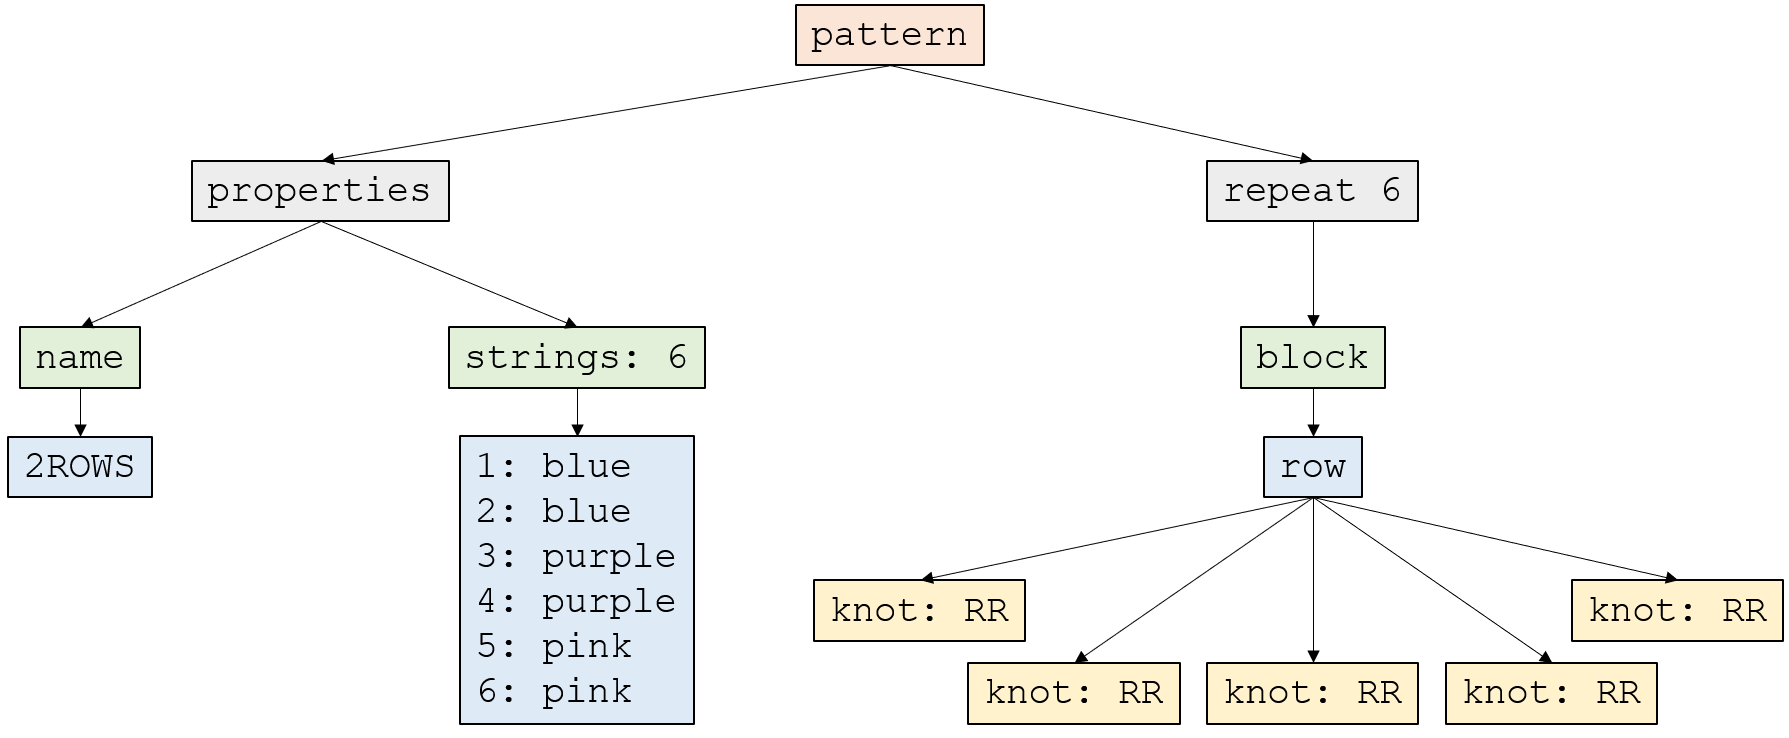
\includegraphics[width=\linewidth]{images/ast1.png}
    \end{center}
    
    \vspace{\baselineskip}
    \textbf{AST for Example 2:}
    \begin{center}
    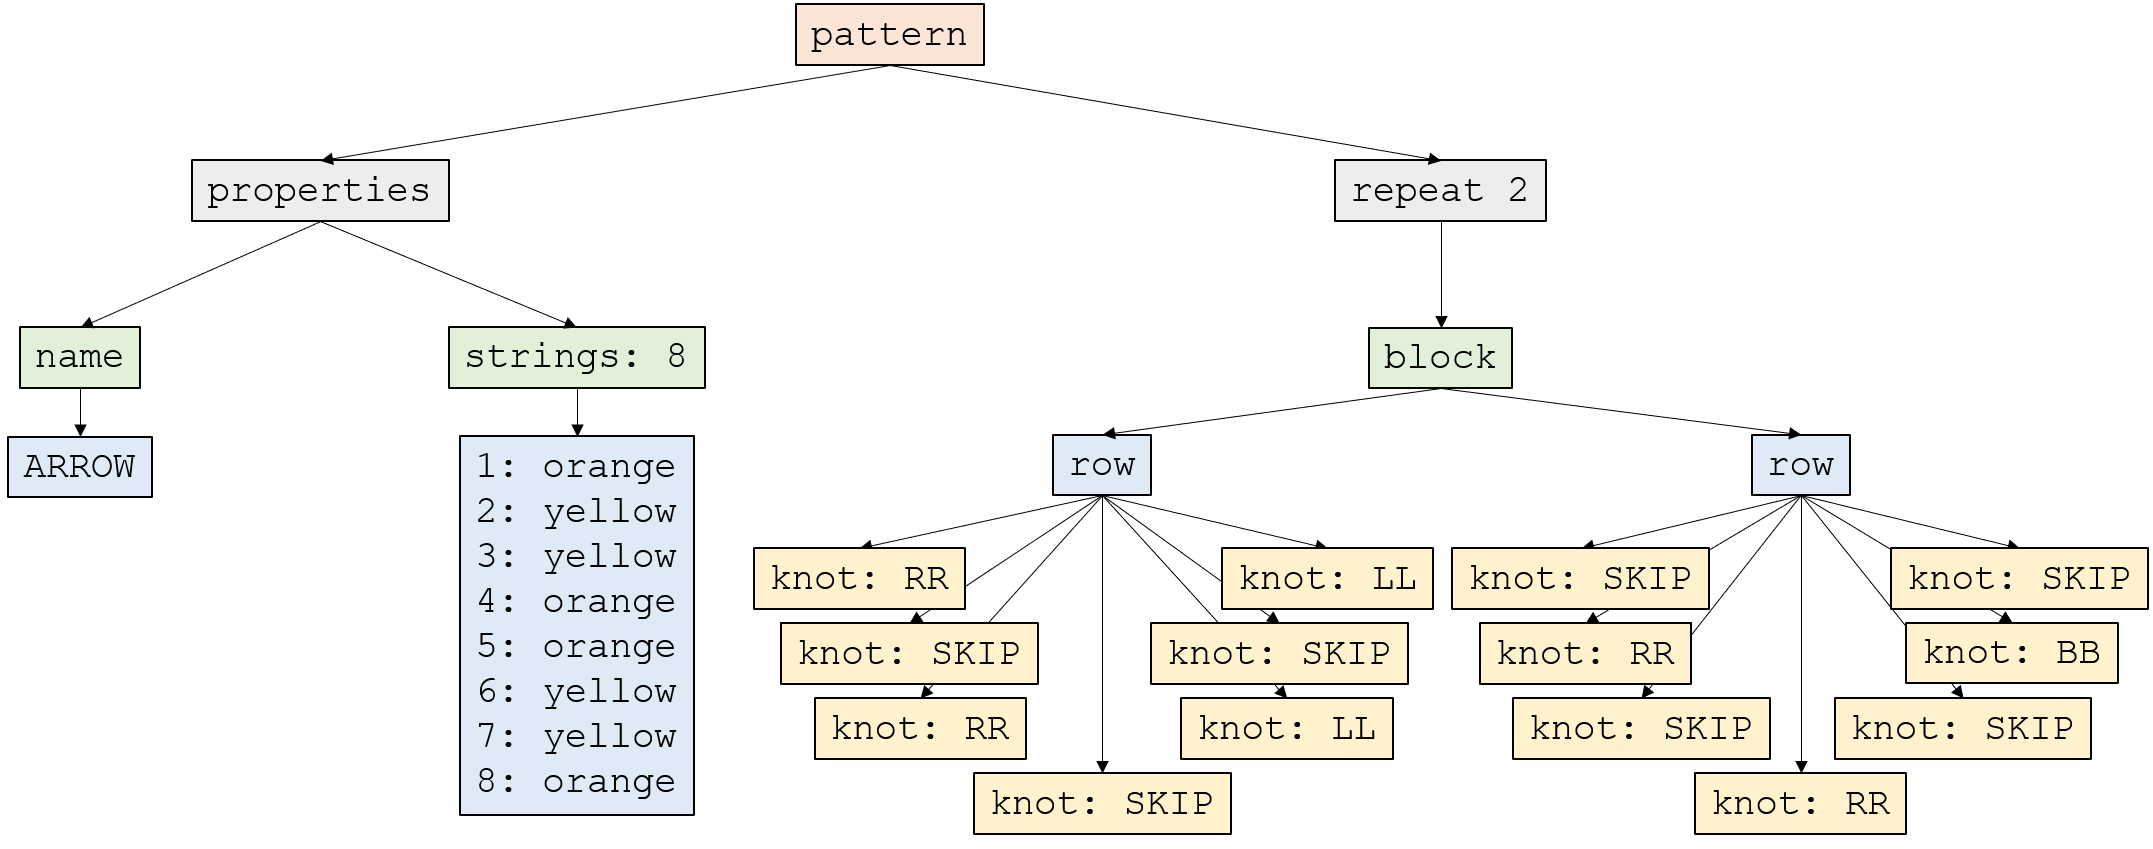
\includegraphics[width=\linewidth]{images/ast2.png}
    \end{center}
    
    \vspace{\baselineskip}
    \textbf{AST for Example 3:}
    \begin{center}
    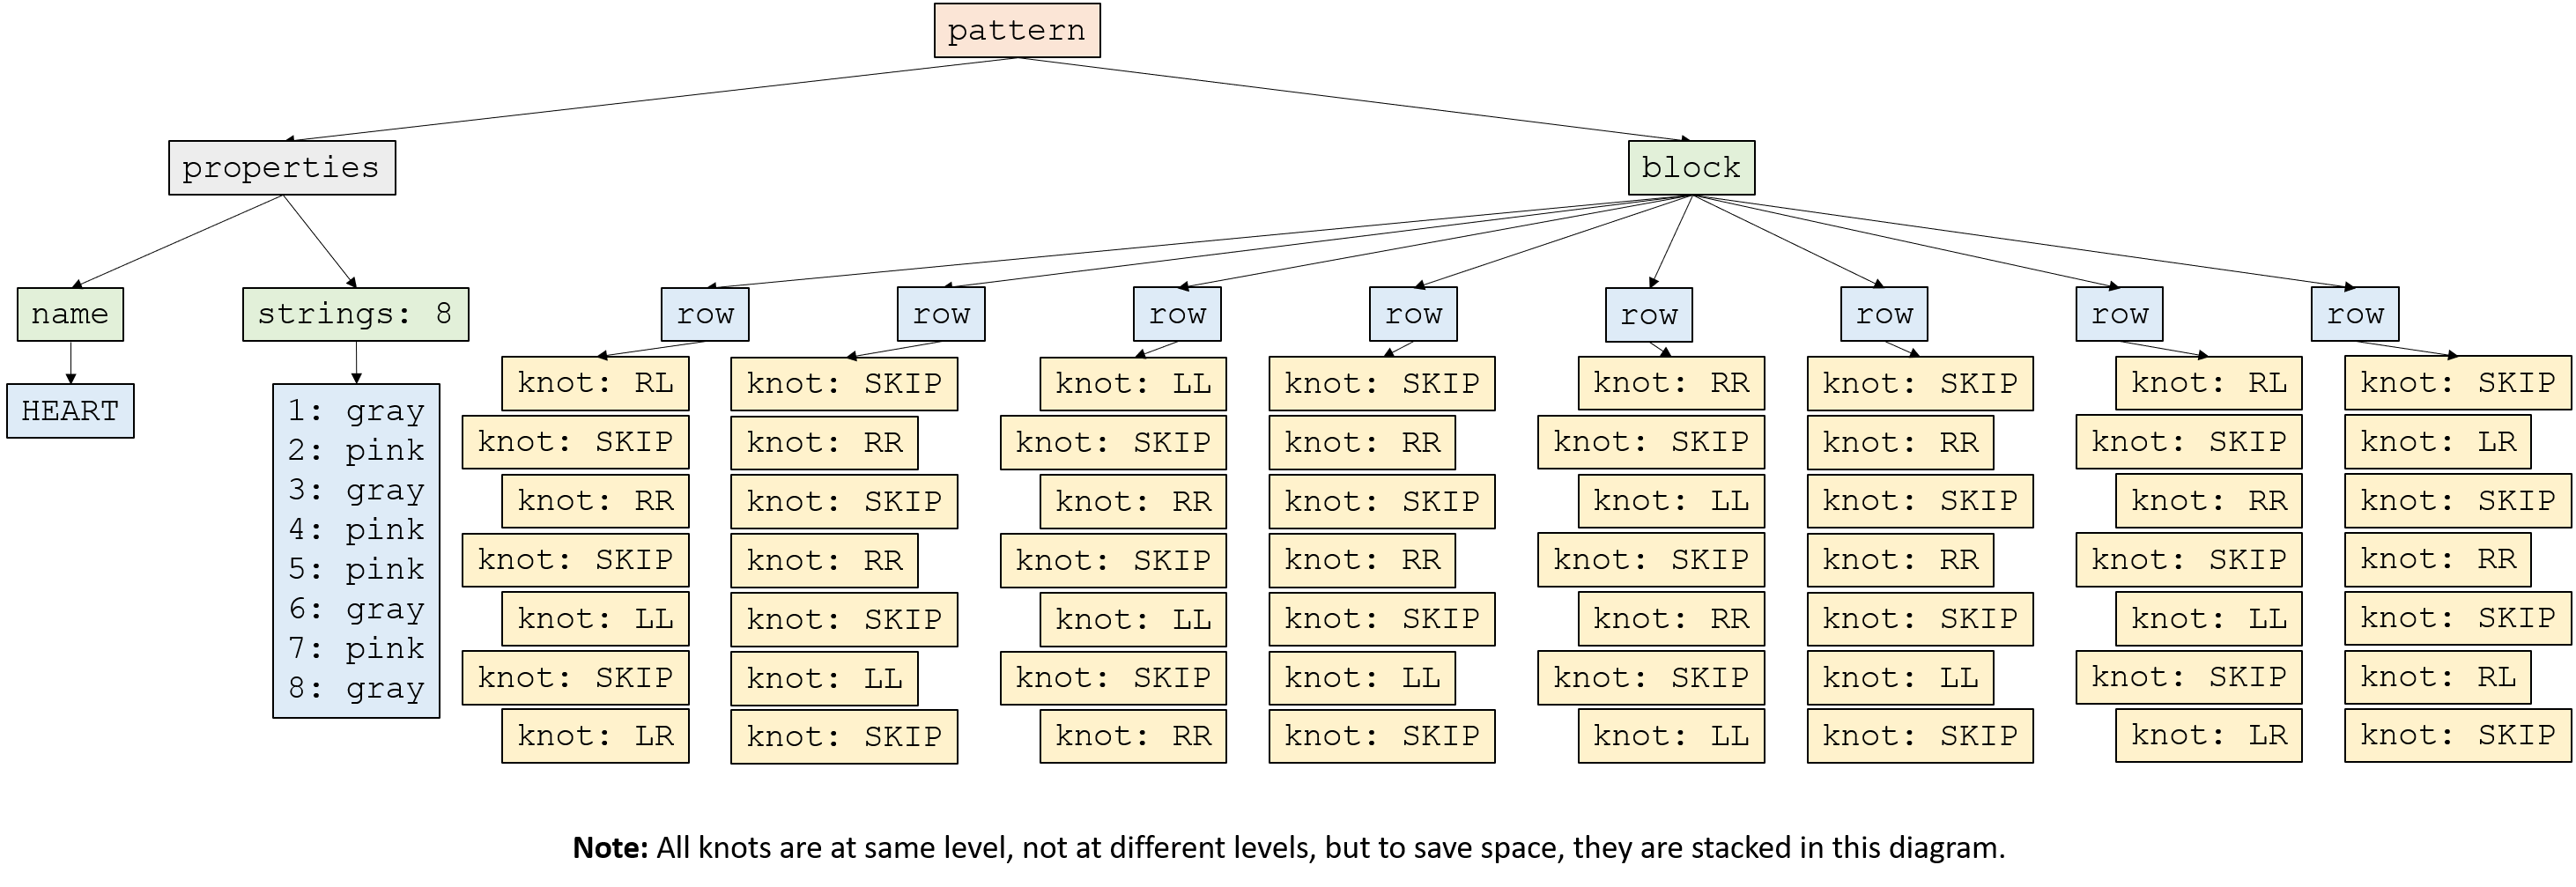
\includegraphics[width=\linewidth]{images/ast3.png}
    \end{center}
    
    \vspace{0.5em}
    \item How is your program evaluated? In particular,
    
    \begin{itemize}
        \item Do programs in your language read any input?
        
        \vspace{0.3em}
        The programs themselves can be inputted as files so the user doesn't have to type everything on the command line. Otherwise, there isn't any input read in by our programs.
        
        \vspace{0.5em}
        \item What is the effect (output) of evaluating a program?
        
        \vspace{0.3em}
        The output will be the pattern created by the user! Ideally, it will be displayed graphically on the screen after their program is complete. We currently plan to generate a svg from the user's program which they can open as a html file.
        
        \vspace{0.5em}
        \item Evaluation is usually conceived of as a depth-first, post-order traversal of an AST. Describe how such a traversal yields the effect you just described and provide illustrations for clarity. Demonstrate evaluation for at least one of your example programs.
        
        \vspace{0.3em}
        A depth-first, post-order traversal of the AST would yield the output described above because this would essentially first evaluate the name and number/colors of strings in the properties subtree, which is needed to evaluate the rest of the pattern. Then, we would evaluate the knots in each row, then the rows in each block, then the blocks themselves, at which point the pattern can be produced since the blocks subtree is now evaluated in full too. 
        
        \vspace{0.3em}
        Here is how evaluation would work for example program 1 (again, the colors are different here, but nothing else should be impacted):
        
        \vspace{\baselineskip}
        
        \begin{center}
	    Step one:
        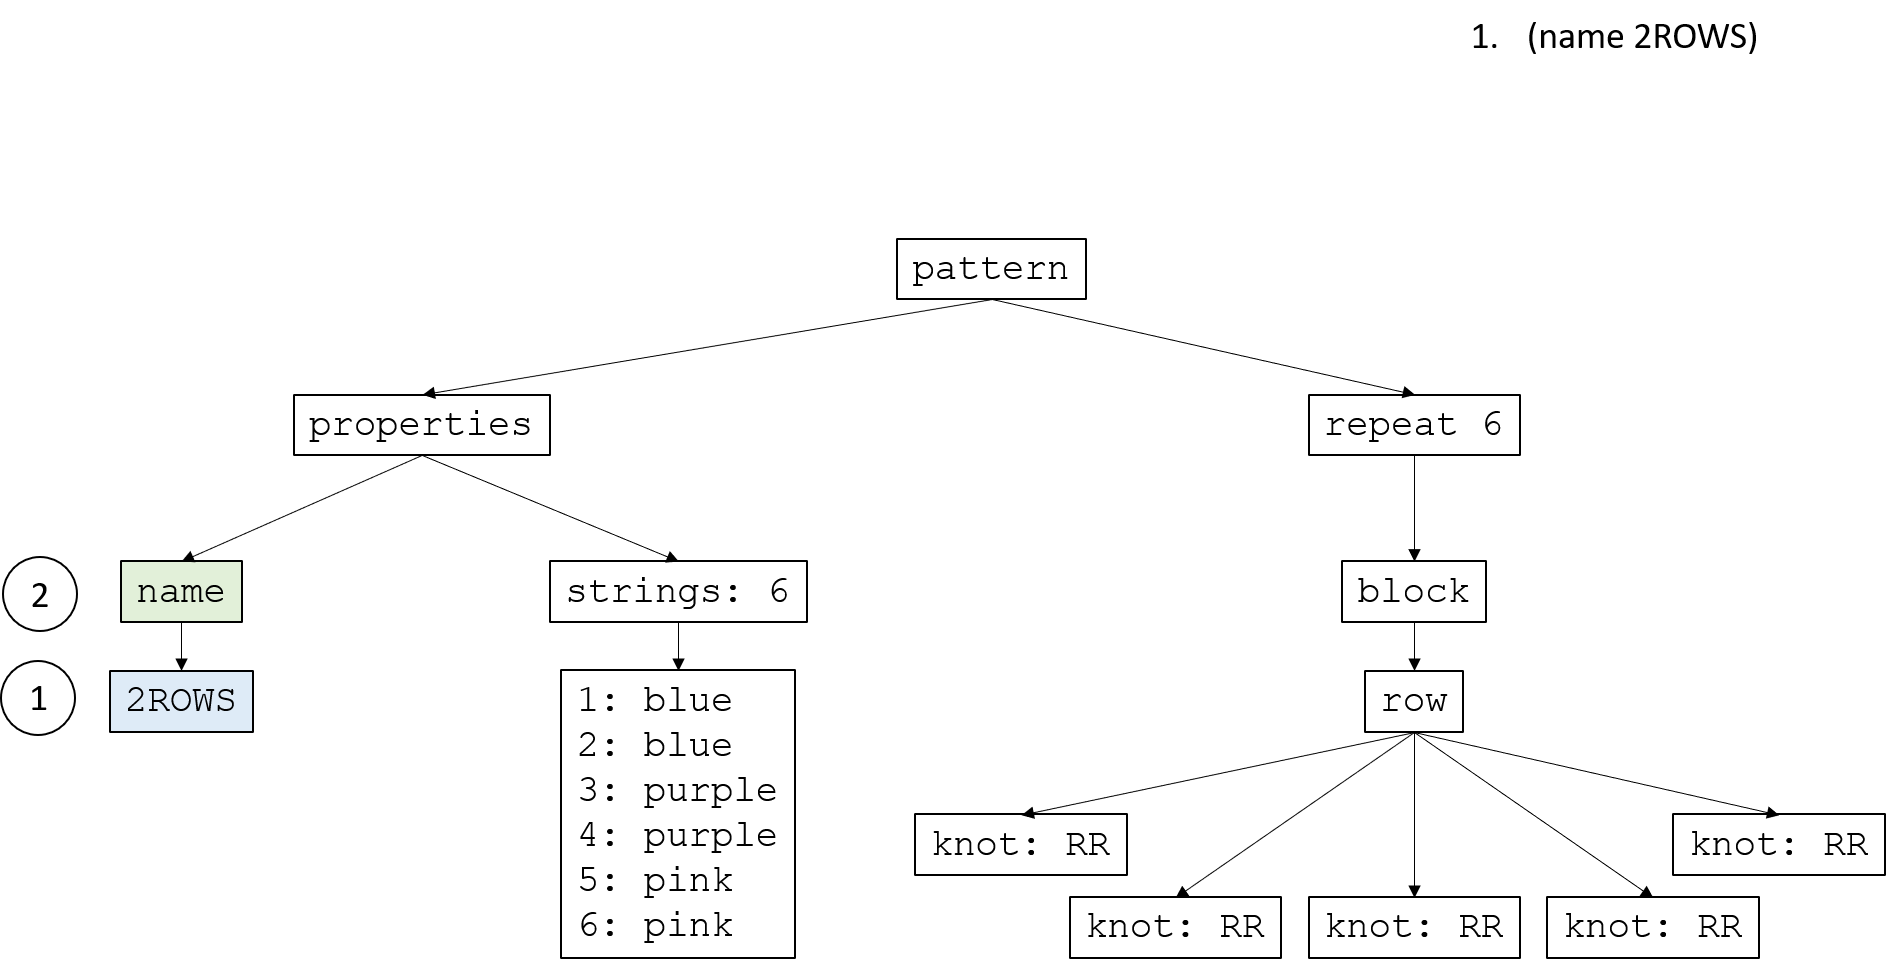
\includegraphics[width=\linewidth]{images/eval1.png}
        
        \vspace{\baselineskip}
        \vspace{\baselineskip}
        Step two:
        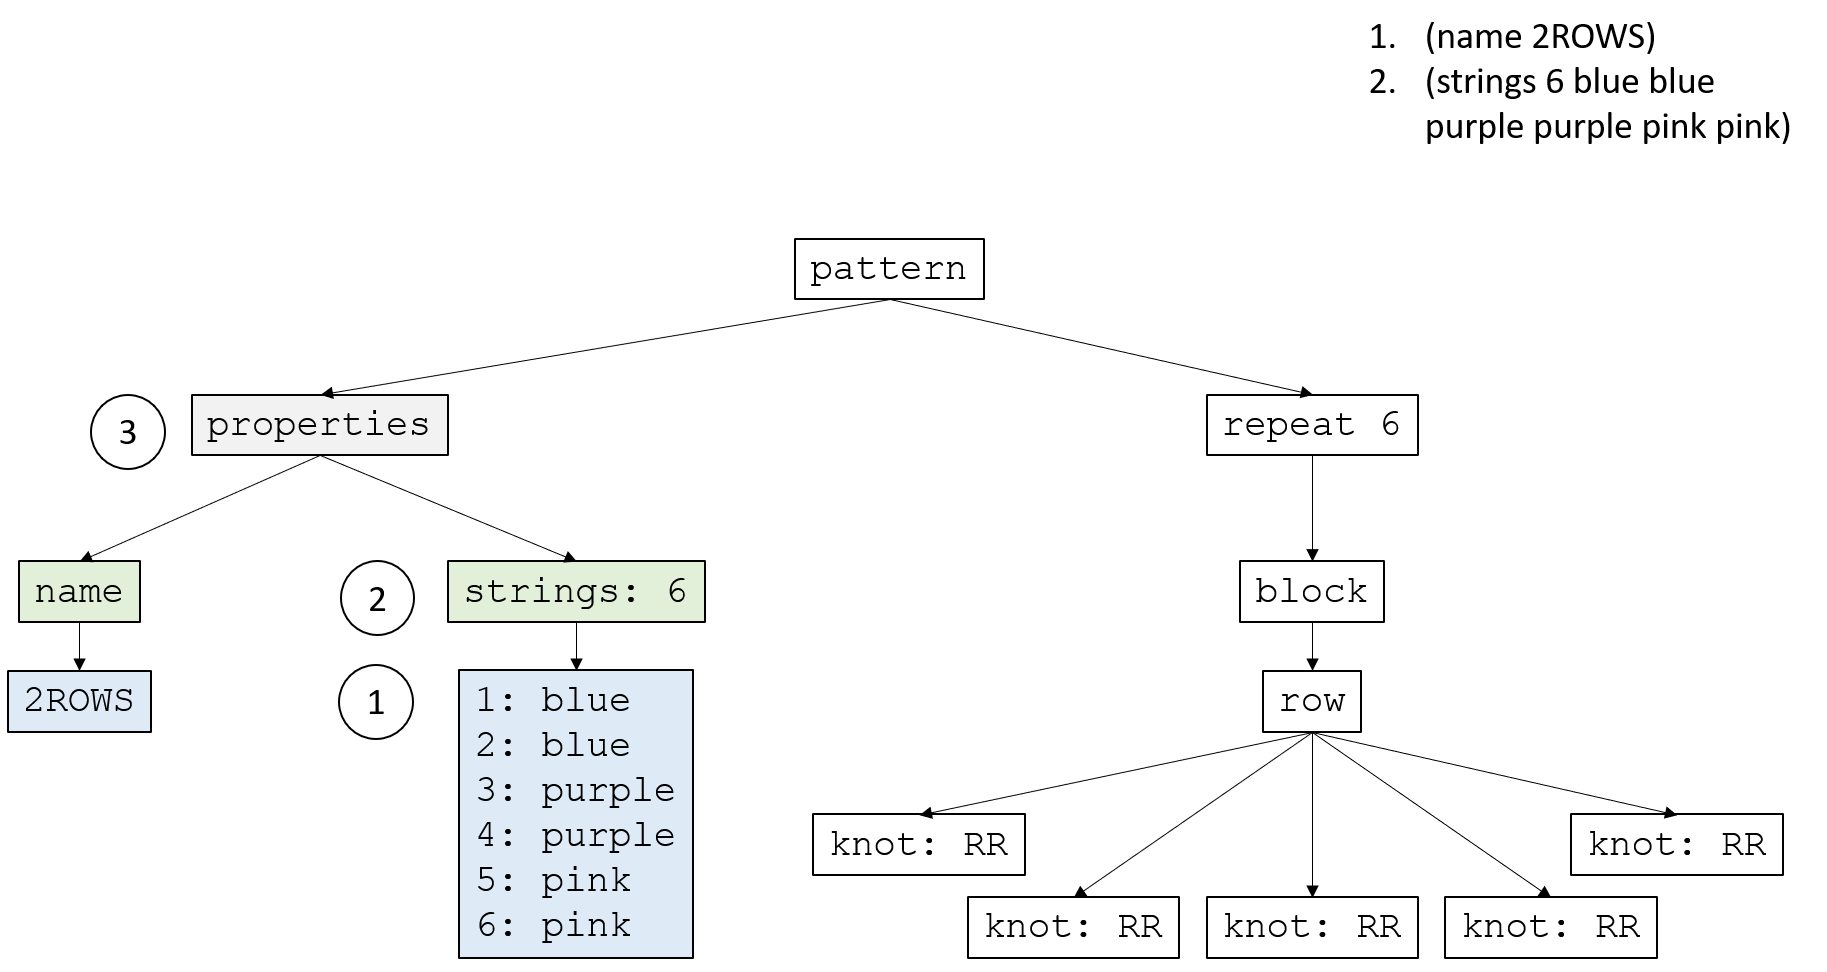
\includegraphics[width=\linewidth]{images/eval2.png}
        
        \vspace{\baselineskip}
        \vspace{\baselineskip}
        Step three:
        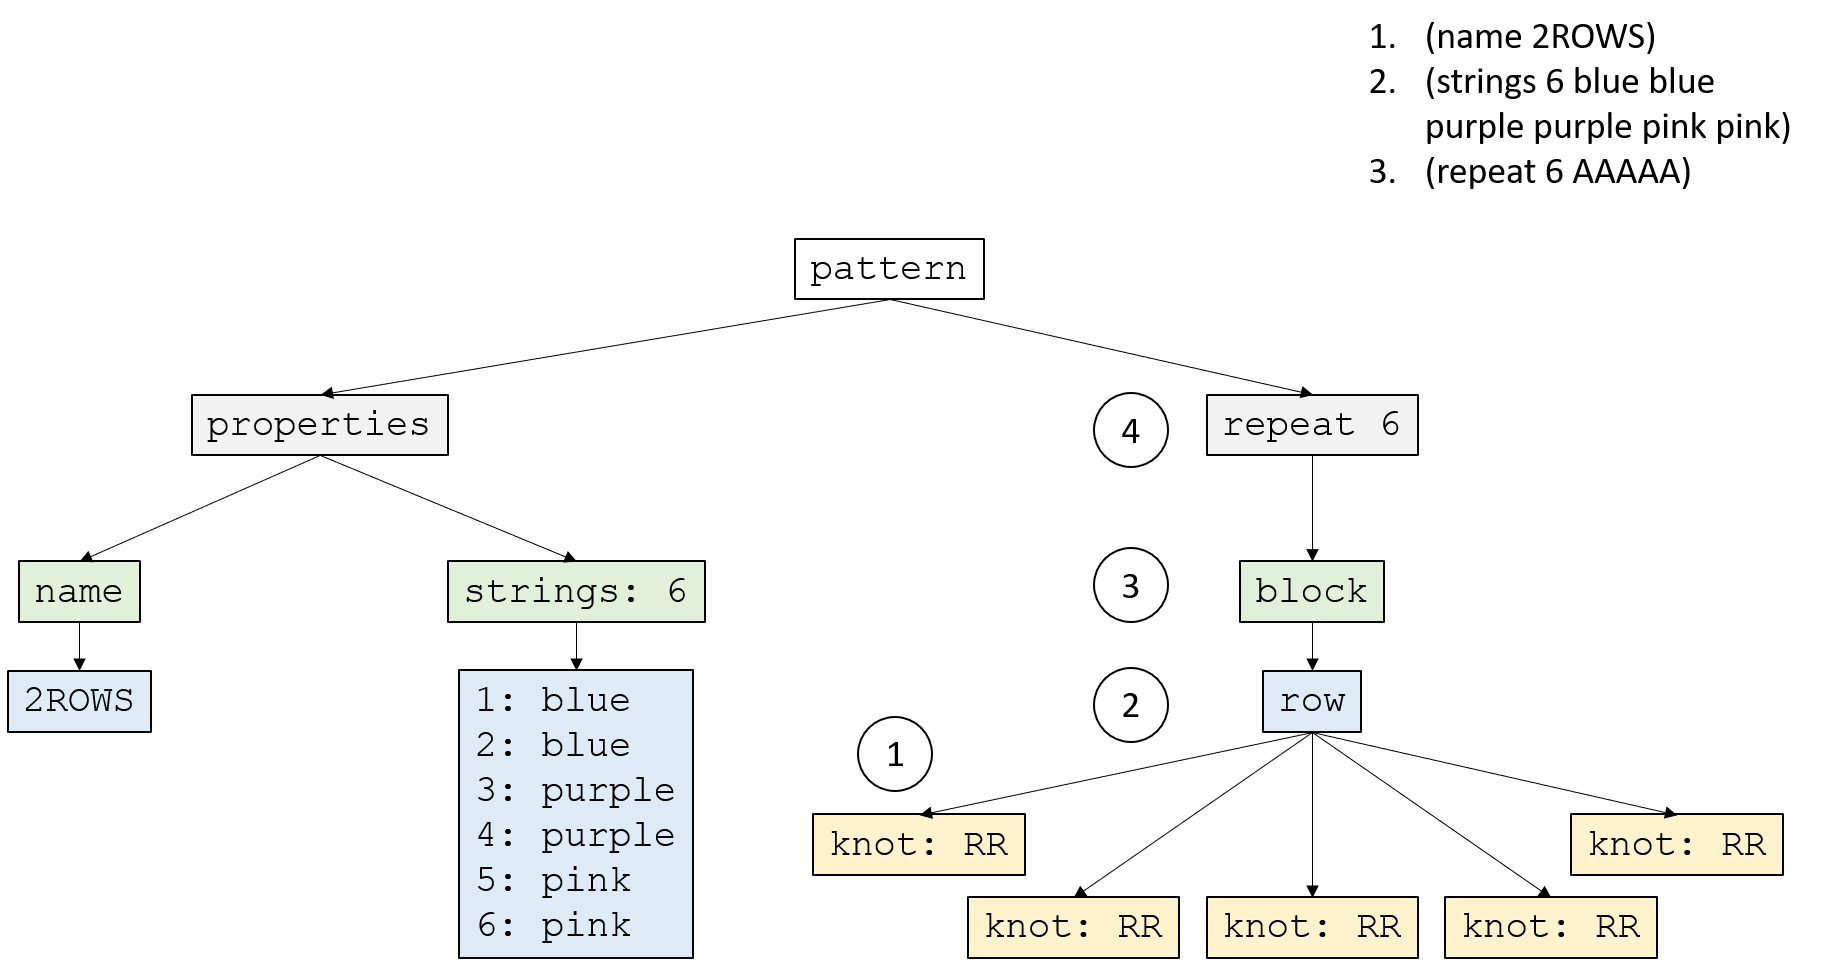
\includegraphics[width=\linewidth]{images/eval3.png}
        
        \vspace{\baselineskip}
        \vspace{\baselineskip}
        Step four:
        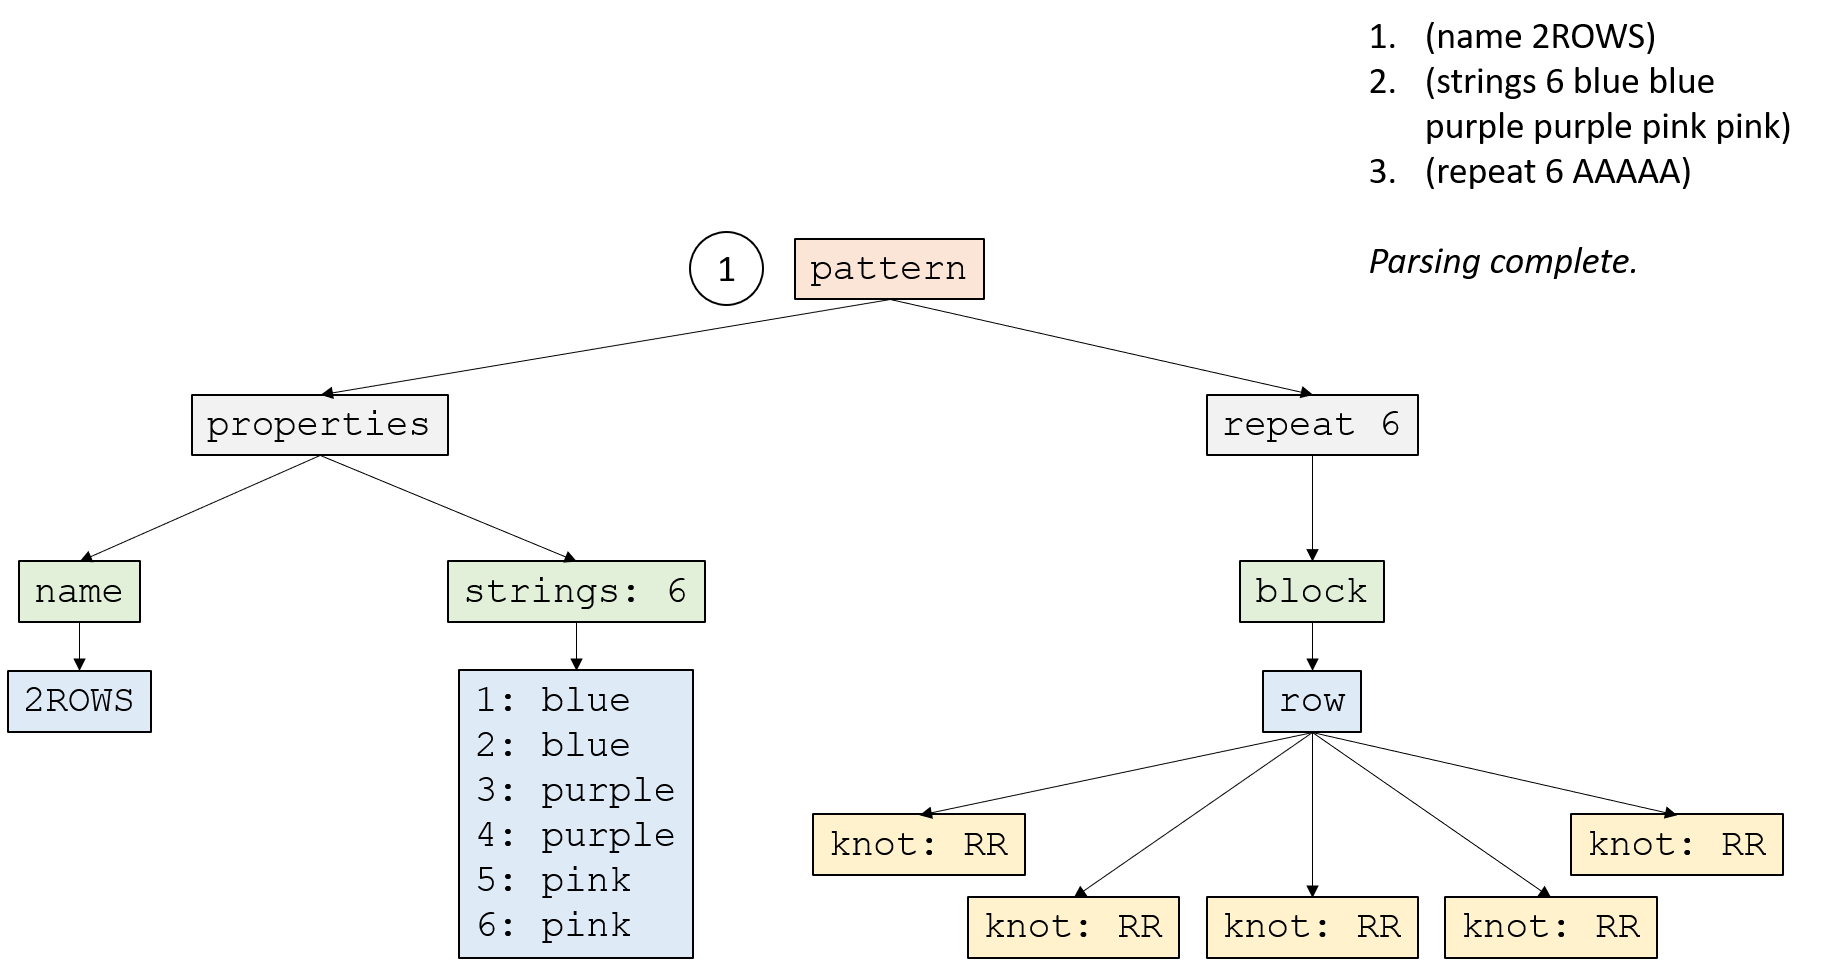
\includegraphics[width=\linewidth]{images/eval4.png}
        \end{center}
	        
	   \end{itemize}
    \end{enumerate}

\section{Remaining Work}

We have basically finished implementing all the necessary operations/data types for our language (and the parser + interpreter are working). For a challenge, we will continuing working on converting the output to svg files and enhancing the resulting graphics.

% DO NOT DELETE ANYTHING BELOW THIS LINE
\end{document}